% Basic document class options
\documentclass[12pt, a4paper]{article}
% Russian locale
\usepackage[T2A]{fontenc}
\usepackage[utf8]{inputenc}
\usepackage[russian]{babel}
% Graphics (images)
\usepackage{graphicx}
\graphicspath{ {images/} }
% Table
\usepackage[table,xcdraw]{xcolor}
\usepackage[tablename=Таблица]{caption}
\usepackage{multirow}
\usepackage{lscape}
% Pictures
\usepackage[figurename=Рисунок]{caption}
\usepackage{ccaption}
\captiondelim{. }

% Title, author and date
\title{МОРФОЛОГИЯ РАКОВИННЫХ АМЕБ РОДА NEBELA ИЗ СФАГНОВЫХ БОЛОТ}
\author{В.А. ЧЕРНЫШОВ}
\date{2008}

\begin{document}
\maketitle % Automatically creating title here.
\begin{abstract}
Задачей настоящего исследования явилось морфологическое изучение популяций 9 видов рода Nebela. Материал был собран летом 2004 г. в разнотипных сфагновых биотопах Пензенской области и Лоухского р-на Карелии.
\end{abstract}

Род Nebela Leidy, 1874 – один из самых крупных среди раковинных амеб [\ref{reference1}, \ref{reference2}], включает около 100 видов. Раковинка у этих корненожек в плане овальная, грушевидная, латерально более или менее уплощенная. На заднем конце и с боков иногда несет валик или киль. Покров из крупных или мелких, круглых, эллиптических, палочковидных, свободно лежащих или перекрывающихся идиосом. Устье от узко- до широкоэллиптического, круглое, прямо срезанное или выпуклое, иногда окружено узким валиком. Раковинка прозрачная, бесцветная или серовато-желтого цвета. Ядро овулярное. Большинство небел являются хищниками, поедают мелких эуглифид. Обитают в сфагнуме и почвах [\ref{reference3}].

В таблице представлены морфометрические показатели исследованных популяций, а ниже приводятся их морфологические описания и изображения.

Nebela (Physochilla) griseola Penard, 1911 (рис. \ref{fig:pic1}.1). Раковинка средняя, в плане грушевидная, поперечное сечение круглое, боковые стороны сходятся по направлению к округлому окруженному валиком устью.

Nebela (Argynnia) dentistoma Penard, 1890 (рис. \ref{fig:pic1}.2).Раковинка относительно крупная, в плане яйцевидная, в профиль уплощенная. Устье эллиптическое, его край образован овальными, неправильной формы идиосомами, создающими впечатление зубчатости. Париетальные идиосомы эллиптические, палочковидные или неправильно округлые, типичные для представителей рода, не перекрывающиеся своими краями.

Nebela (Argynnia) vitraea Penard, 1899 (рис. \ref{fig:pic1}.3). Раковинка крупная, в плане широкояйцевидная, резко сужается к устью, уплощенная. Идиосомы овальные, круглые и удлиненные, между основными пластинками имеются маленькие, заходящие за края больших. Устье круглое, окружено более крупными, чем на остальной поверхности, закругленными идиосомами, создающими впечатление зубчатости.

Nebela carinata (Archer, 1867) Leidy, 1879 (рис. \ref{fig:pic1}.4). Раковинка крупная, в плане широкогрушевидная, фундус окружен плоским и широким (до 15 мкм) гребнем, продолжающимся до передней трети высоты. Поперечное сечение и устье эллиптические. Идиосомы широкоэллиптические, круглые или многоугольные, на гребне более мелкие, в световой микроскоп выглядят как грубая зернистость. Могут быть латеральные поры в передней трети раковинки. 

Nebela galeata Penard, 1902 (рис. \ref{fig:pic1}.5). Раковинка крупная, прозрачная, бесцветная, в плане грушевидная, в профиль уплощенная. По периметру фундуса до передней трети раковинка окружена краевым валиком. Покрыта круглыми, широкоэллиптическими или неправильной формы идиосомами. Валик сложен преимущественно эллиптическими, одинаковыми или чуть большими, чем на основной части идиосомами. Устье широкоэллиптическое. В передней трети раковинки могут быть латеральные поры.

Nebela marginata Penard, 1902 (рис. \ref{fig:pic1}.6). Раковинка крупная, в плане широкогрушевидная, в профиль узкоэллиптическая. До передней трети раковинки по латеральной кайме проходит очень узкий (2–4 мкм) гребень, покрытый более мелкими, по сравнению со всей раковинкой, эллиптическими, полигональными или палочковидными идиосомами. Устье эллиптическое. 

Nebela maxima Awerintzew, 1907 (рис. \ref{fig:pic1}.7). Раковинка очень крупная, в плане удлиненнояйцевидная. От середины фундуса по всей его периферии располагаются не очень широкий гребень с неровными краями. Устье овальное, окружено губой органического вещества.

Nebela parvula Cash, 1909  (рис. \ref{fig:pic1}.8) Раковинка относительно крупная, в плане яйцевидная, фундус сферический постепенно сужается по направлению к устью. Устье с прямым контуром, окружено губой органического вещества.

Nebelatincta (Leidy, 1879) Awerintzew, 1906 (рис. \ref{fig:pic1}.9). Раковинка относительно крупная, в плане грушевидная или яйцевидная, латерально уплощенная. По бокам невдалеке от эллиптического устья две дополнительные поры, не всегда четко выраженные. Мелкие идиосомы иногда покрывают только часть раковинки, что создает сходство с видами Hyalosphenia.

Наиболее вариабельные виды – Nebela tincta и Nebela vitraea. Наименее изменчивый вид – Nebela
marginata.

\begin{figure}[h]
    \centering
    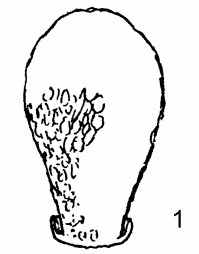
\includegraphics[width=0.15\textwidth]{1.png}
    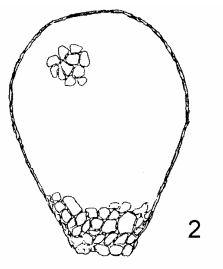
\includegraphics[width=0.15\textwidth]{2.png}
    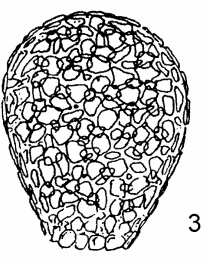
\includegraphics[width=0.15\textwidth]{3.png}
    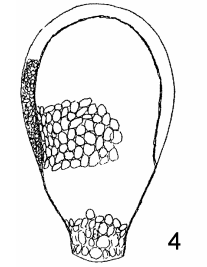
\includegraphics[width=0.15\textwidth]{4.png}
    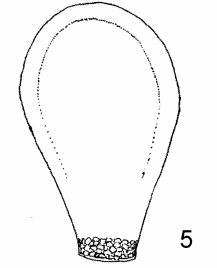
\includegraphics[width=0.15\textwidth]{5.png}
    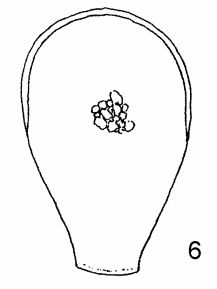
\includegraphics[width=0.15\textwidth]{6.png}
    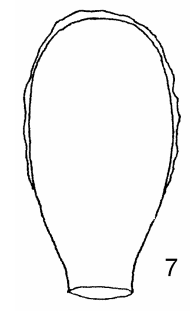
\includegraphics[width=0.15\textwidth]{7.png}
    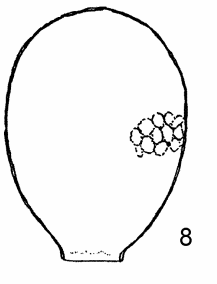
\includegraphics[width=0.15\textwidth]{8.png}
    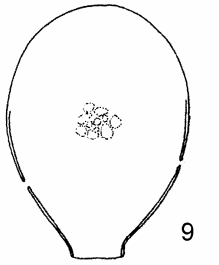
\includegraphics[width=0.15\textwidth]{9.png}
    \caption{Представители разных видов рода Nebela. 
    \\*
    1 – N. (Physochilla) griseola, 2 – N. (Argynnia) dentistoma, 3 – N. (Argynnia) vitraea, 4 – N. carinata, 5 – N. galeata, 6 – N. marginata, 7 – N. maxima, 8 – N. parvula, 9 – N. tincta.
    }
    \label{fig:pic1}
\end{figure}


\begin{table}[h]
\caption{Морфометрическая характеристика исследованных популяций (1 – длина раковинки, 2 – ширина раковинки, 3 – ширина устья)}
\label{tab:table}
\resizebox{\columnwidth}{!}{%
\begin{tabular}{|llllllll|}
\hline
\multicolumn{1}{|c|}{\multirow{2}{*}{Вид и параметр раковинки}} & \multicolumn{7}{c|}{Морфологический показатель}                                                                                                                                                                                                                                                             \\ \cline{2-8} 
\multicolumn{1}{|c|}{}                                          & \multicolumn{1}{c|}{\rotatebox[origin=c]{90}{Среднее арифметическое, мкм}} & \multicolumn{1}{c|}{\rotatebox[origin=c]{90}{Медиана, мкм}} & \multicolumn{1}{c|}{\rotatebox[origin=c]{90}{Стандартное отклонение, мкм}} & \multicolumn{1}{c|}{\rotatebox[origin=c]{90}{Ошибка средней, мкм}} & \multicolumn{1}{c|}{\rotatebox[origin=c]{90}{Коэффициент вариации, \%}} & \multicolumn{1}{c|}{\rotatebox[origin=c]{90}{Минимум, мкм}} & \multicolumn{1}{c|}{\rotatebox[origin=c]{90}{Максимум, мкм}} \\ \hline
\multicolumn{8}{|l|}{Nebela (Physochilla) griseola}                                                                                                                                                                                                                                                                                                                           \\ \hline
\multicolumn{1}{|l|}{1}                                         & \multicolumn{1}{l|}{75.7}                        & \multicolumn{1}{l|}{73.4}         & \multicolumn{1}{l|}{8.1}                         & \multicolumn{1}{l|}{1.8}                 & \multicolumn{1}{l|}{10.7}                     & \multicolumn{1}{l|}{65.1}         & 97.7                               \\ \hline
\multicolumn{1}{|l|}{2}                                         & \multicolumn{1}{l|}{53.1}                        & \multicolumn{1}{l|}{52.7}         & \multicolumn{1}{l|}{7.0}                         & \multicolumn{1}{l|}{1.6}                 & \multicolumn{1}{l|}{13.2}                     & \multicolumn{1}{l|}{37.0}         & 64.8                               \\ \hline
\multicolumn{1}{|l|}{3}                                         & \multicolumn{1}{l|}{20.3}                        & \multicolumn{1}{l|}{20.6}         & \multicolumn{1}{l|}{2.3}                         & \multicolumn{1}{l|}{0.5}                 & \multicolumn{1}{l|}{11.4}                     & \multicolumn{1}{l|}{16.1}         & 23.6                               \\ \hline
\multicolumn{8}{|l|}{Nebela (Argynnia) dentistoma}                                                                                                                                                                                                                                                                                                                            \\ \hline
\multicolumn{1}{|l|}{1}                                         & \multicolumn{1}{l|}{75.7}                        & \multicolumn{1}{l|}{73.4}         & \multicolumn{1}{l|}{8.1}                         & \multicolumn{1}{l|}{1.8}                 & \multicolumn{1}{l|}{10.7}                     & \multicolumn{1}{l|}{65.1}         & 97.7                               \\ \hline
\multicolumn{1}{|l|}{2}                                         & \multicolumn{1}{l|}{53.1}                        & \multicolumn{1}{l|}{52.7}         & \multicolumn{1}{l|}{7.0}                         & \multicolumn{1}{l|}{1.6}                 & \multicolumn{1}{l|}{13.2}                     & \multicolumn{1}{l|}{37.0}         & 64.8                               \\ \hline
\multicolumn{1}{|l|}{3}                                         & \multicolumn{1}{l|}{20.3}                        & \multicolumn{1}{l|}{20.6}         & \multicolumn{1}{l|}{2.3}                         & \multicolumn{1}{l|}{0.5}                 & \multicolumn{1}{l|}{11.4}                     & \multicolumn{1}{l|}{16.1}         & 23.6                               \\ \hline
\multicolumn{8}{|l|}{Nebela (Argynnia) vitraea}                                                                                                                                                                                                                                                                                                                               \\ \hline
\multicolumn{1}{|l|}{1}                                         & \multicolumn{1}{l|}{155.5}                       & \multicolumn{1}{l|}{158.0}        & \multicolumn{1}{l|}{17.1}                        & \multicolumn{1}{l|}{3.8}                 & \multicolumn{1}{l|}{11.0}                     & \multicolumn{1}{l|}{119.3}        & 180.7                              \\ \hline
\multicolumn{1}{|l|}{2}                                         & \multicolumn{1}{l|}{128.1}                       & \multicolumn{1}{l|}{129.2}        & \multicolumn{1}{l|}{19.2}                        & \multicolumn{1}{l|}{4.3}                 & \multicolumn{1}{l|}{15.0}                     & \multicolumn{1}{l|}{83.0}         & 155.8                              \\ \hline
\multicolumn{1}{|l|}{3}                                         & \multicolumn{1}{l|}{37.0}                        & \multicolumn{1}{l|}{36.4}         & \multicolumn{1}{l|}{5.5}                         & \multicolumn{1}{l|}{1.2}                 & \multicolumn{1}{l|}{14.8}                     & \multicolumn{1}{l|}{26.7}         & 45.1                               \\ \hline
\multicolumn{8}{|l|}{Nebela carinata}                                                                                                                                                                                                                                                                                                                                         \\ \hline
\multicolumn{1}{|l|}{1}                                         & \multicolumn{1}{l|}{192.8}                       & \multicolumn{1}{l|}{191.8}        & \multicolumn{1}{l|}{10.7}                        & \multicolumn{1}{l|}{2.4}                 & \multicolumn{1}{l|}{5.6}                      & \multicolumn{1}{l|}{172.9}        & 216.8                              \\ \hline
\multicolumn{1}{|l|}{2}                                         & \multicolumn{1}{l|}{125.4}                       & \multicolumn{1}{l|}{122.6}        & \multicolumn{1}{l|}{12.7}                        & \multicolumn{1}{l|}{2.9}                 & \multicolumn{1}{l|}{10.2}                     & \multicolumn{1}{l|}{102.0}        & 150.5                              \\ \hline
\multicolumn{1}{|l|}{3}                                         & \multicolumn{1}{l|}{40.8}                        & \multicolumn{1}{l|}{40.8}         & \multicolumn{1}{l|}{2.9}                         & \multicolumn{1}{l|}{0.7}                 & \multicolumn{1}{l|}{7.1}                      & \multicolumn{1}{l|}{34.5}         & 46.8                               \\ \hline
\multicolumn{8}{|l|}{Nebela galeata}                                                                                                                                                                                                                                                                                                                                          \\ \hline
\multicolumn{1}{|l|}{1}                                         & \multicolumn{1}{l|}{219.5}                       & \multicolumn{1}{l|}{216.2}        & \multicolumn{1}{l|}{15.0}                        & \multicolumn{1}{l|}{3.4}                 & \multicolumn{1}{l|}{6.8}                      & \multicolumn{1}{l|}{194.9}        & 247.7                              \\ \hline
\multicolumn{1}{|l|}{2}                                         & \multicolumn{1}{l|}{133.5}                       & \multicolumn{1}{l|}{124.3}        & \multicolumn{1}{l|}{20.8}                        & \multicolumn{1}{l|}{4.7}                 & \multicolumn{1}{l|}{15.6}                     & \multicolumn{1}{l|}{112.5}        & 177.3                              \\ \hline
\multicolumn{1}{|l|}{3}                                         & \multicolumn{1}{l|}{44.4}                        & \multicolumn{1}{l|}{44.7}         & \multicolumn{1}{l|}{3.0}                         & \multicolumn{1}{l|}{0.7}                 & \multicolumn{1}{l|}{6.8}                      & \multicolumn{1}{l|}{38.6}         & 48.6                               \\ \hline
\multicolumn{8}{|l|}{Nebela marginata}                                                                                                                                                                                                                                                                                                                                        \\ \hline
\multicolumn{1}{|l|}{1}                                         & \multicolumn{1}{l|}{182.2}                       & \multicolumn{1}{l|}{181.6}        & \multicolumn{1}{l|}{7.4}                         & \multicolumn{1}{l|}{1.7}                 & \multicolumn{1}{l|}{4.1}                      & \multicolumn{1}{l|}{168}          & 199.7                              \\ \hline
\multicolumn{1}{|l|}{2}                                         & \multicolumn{1}{l|}{122.8}                       & \multicolumn{1}{l|}{122.5}        & \multicolumn{1}{l|}{5.7}                         & \multicolumn{1}{l|}{1.3}                 & \multicolumn{1}{l|}{4.6}                      & \multicolumn{1}{l|}{110.7}        & 132.1                              \\ \hline
\multicolumn{1}{|l|}{3}                                         & \multicolumn{1}{l|}{45.9}                        & \multicolumn{1}{l|}{45.7}         & \multicolumn{1}{l|}{3.0}                         & \multicolumn{1}{l|}{0.7}                 & \multicolumn{1}{l|}{6.5}                      & \multicolumn{1}{l|}{40.6}         & 50.1                               \\ \hline
\multicolumn{8}{|l|}{Nebela maxima}                                                                                                                                                                                                                                                                                                                                           \\ \hline
\multicolumn{1}{|l|}{1}                                         & \multicolumn{1}{l|}{233.0}                       & \multicolumn{1}{l|}{224.7}        & \multicolumn{1}{l|}{25.5}                        & \multicolumn{1}{l|}{5.7}                 & \multicolumn{1}{l|}{10.9}                     & \multicolumn{1}{l|}{203.7}        & 282.8                              \\ \hline
\multicolumn{1}{|l|}{2}                                         & \multicolumn{1}{l|}{133.5}                       & \multicolumn{1}{l|}{128.4}        & \multicolumn{1}{l|}{15.0}                        & \multicolumn{1}{l|}{3.4}                 & \multicolumn{1}{l|}{11.2}                     & \multicolumn{1}{l|}{113.4}        & 171.2                              \\ \hline
\multicolumn{1}{|l|}{3}                                         & \multicolumn{1}{l|}{48.4}                        & \multicolumn{1}{l|}{48.5}         & \multicolumn{1}{l|}{4.8}                         & \multicolumn{1}{l|}{1.1}                 & \multicolumn{1}{l|}{9.9}                      & \multicolumn{1}{l|}{38.2}         & 55.7                               \\ \hline
\multicolumn{8}{|l|}{Nebela parvula}                                                                                                                                                                                                                                                                                                                                          \\ \hline
\multicolumn{1}{|l|}{1}                                         & \multicolumn{1}{l|}{86.8}                        & \multicolumn{1}{l|}{85.6}         & \multicolumn{1}{l|}{7.3}                         & \multicolumn{1}{l|}{1.6}                 & \multicolumn{1}{l|}{8.4}                      & \multicolumn{1}{l|}{72.1}         & 103.8                              \\ \hline
\multicolumn{1}{|l|}{2}                                         & \multicolumn{1}{l|}{62.3}                        & \multicolumn{1}{l|}{60.8}         & \multicolumn{1}{l|}{6.1}                         & \multicolumn{1}{l|}{1.4}                 & \multicolumn{1}{l|}{9.7}                      & \multicolumn{1}{l|}{55.2}         & 82.4                               \\ \hline
\multicolumn{1}{|l|}{3}                                         & \multicolumn{1}{l|}{20.8}                        & \multicolumn{1}{l|}{20.1}         & \multicolumn{1}{l|}{2.5}                         & \multicolumn{1}{l|}{0.6}                 & \multicolumn{1}{l|}{12.1}                     & \multicolumn{1}{l|}{18.5}         & 28.8                               \\ \hline
\multicolumn{8}{|l|}{Nebela tincta}                                                                                                                                                                                                                                                                                                                                           \\ \hline
\multicolumn{1}{|l|}{1}                                         & \multicolumn{1}{l|}{93.1}                        & \multicolumn{1}{l|}{90}           & \multicolumn{1}{l|}{14.6}                        & \multicolumn{1}{l|}{3.3}                 & \multicolumn{1}{l|}{15.7}                     & \multicolumn{1}{l|}{76.0}         & 141.4                              \\ \hline
\multicolumn{1}{|l|}{2}                                         & \multicolumn{1}{l|}{67.3}                        & \multicolumn{1}{l|}{64.1}         & \multicolumn{1}{l|}{11.7}                        & \multicolumn{1}{l|}{2.6}                 & \multicolumn{1}{l|}{17.3}                     & \multicolumn{1}{l|}{50.9}         & 107.1                              \\ \hline
\multicolumn{1}{|l|}{3}                                         & \multicolumn{1}{l|}{22.0}                        & \multicolumn{1}{l|}{20.6}         & \multicolumn{1}{l|}{5.0}                         & \multicolumn{1}{l|}{1.1}                 & \multicolumn{1}{l|}{22.9}                     & \multicolumn{1}{l|}{18.5}         & 41.6                               \\ \hline
\end{tabular}%
}
\end{table}

\section*{Список литературы:}

\begin{enumerate}
  \item Мазей Ю. А., Цыганов А. Н. Пресноводные раковинные амёбы. М.: Товарищество научных изданий КМК, 2006. 300 с. \label{reference1}
  \item Deflandre G. Etude monographique sur le genre Nebela Leidy (Rhizopoda-Testacea) // Ann. Protistol. 1936. T. 5. P. 201–322. \label{reference2}
  \item Ogden C. G., Hedley R. H. An atlas of freshwater testate amoebae. London: Oxford Univ. Press, 1980. 222 pp. \label{reference3}
\end{enumerate}

\end{document}
